% FEEDBACK
%
% !TEX root = ../thesis-main.tex
%
\chapter{Feedback on lexical stress errors}
\label{chap:feedback}

%\cleanchapterquote{You can’t do better design with a computer, but you can speed up your work enormously.}{Wim Crouwel}{(Graphic designer and typographer)}

 

\begin{figure}[htb]
		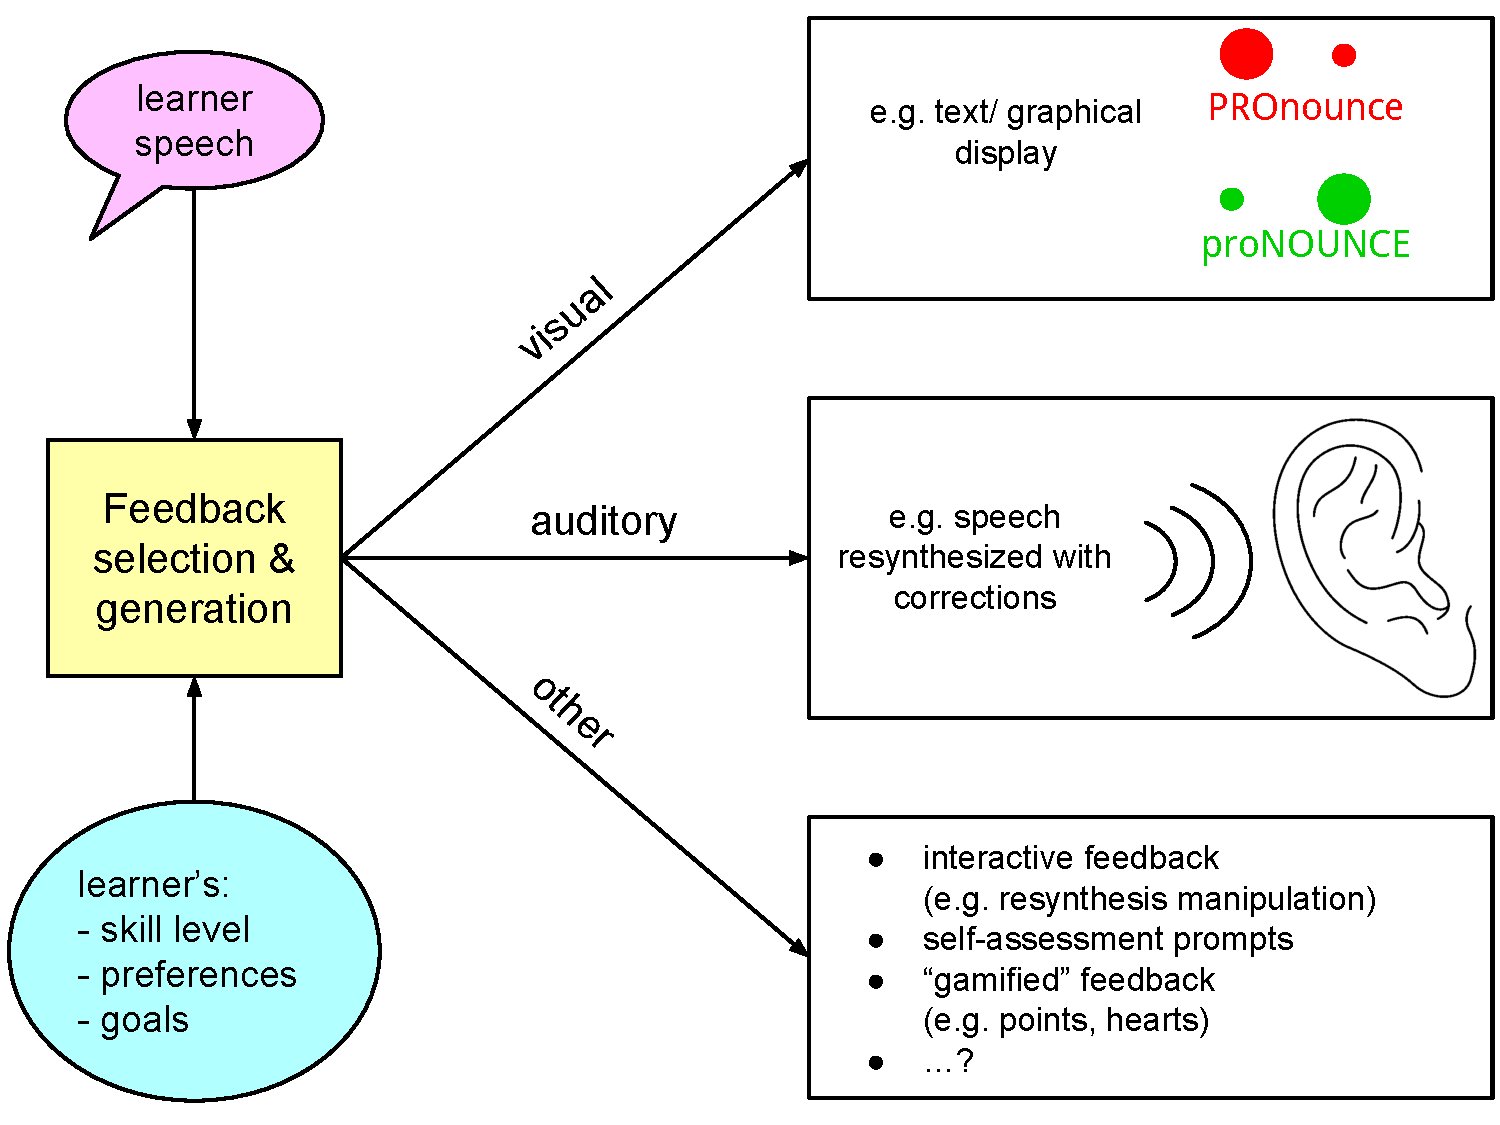
\includegraphics[width=\textwidth]{../img/feedback}
		\caption{Delivery of prosody feedback in different modalities.}
		\label{fig:feedback}
	\end{figure}

\section{Related work}
\label{sec:fb:related}

	\cite{Sitaram2011}
	\cite{Bonneau2011}
	\citep{Hattie2007}
	

\section{Visual feedback}
\label{sec:fb:visual}

	\subsection{Stylized text}
	\label{sec:visual:text}
	
	\subsection{Graphical representations of prosody}
	\label{sec:visual:graphics}
	
	\subsection{Visualizations of the speech signal}
	\label{sec:visual:visualizations}
	
	
	
\section{Auditory feedback}
\label{sec:fb:auditory}

	\subsection{Enhanced reference utterance}
	\label{sec:auditory:enhanced}
	
	\subsection{Resynthesized learner speech}
	\label{sec:auditory:resynth}
	
	
	
\section{Alternative feedback types}
\label{sec:fb:alternative}

	\subsection{Metalinguistic feedback}
	\label{sec:alternative:metaling}
	
	\subsection{Interactive feedback}
	\label{sec:alternative:interactive}
	
	\subsection{Implicit feedback}
	\label{sec:alternative:implicit}

\section{Summary}
\label{sec:fb:summary}